\documentclass[../main.tex]
		
		\begin{document}
			\section{Composition of Functions}
	\begin{description}
		\item[Task:] Understand the natural operation that allows us to combine functions.
		\begin{figure}[h]
			\centering
			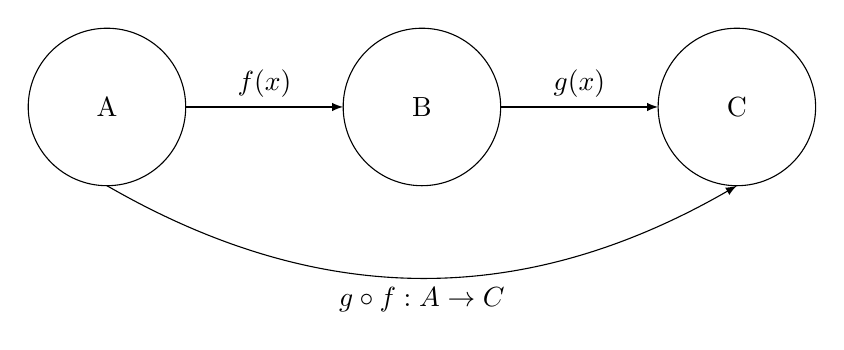
\begin{tikzpicture}
				\coordinate (A) at (-4, 0);
				\coordinate (B) at (0, 0);
				\coordinate (C) at (4, 0);
				
				\draw {(A) circle (1)} node{A};
				\draw {(B) circle (1)} node{B};
				\draw {(C) circle (1)} node{C};
				
				\draw [-latex](-3, 0) -- (-2, 0) node[above]{$f(x)$} -- (-1, 0);
				\draw [-latex](1, 0) -- (2, 0) node[above]{$g(x)$} -- (3, 0);
				\draw [-latex](-4, -1) to[bend right] node[below]{$g \circ f: A \rightarrow C$} (4, -1);
			\end{tikzpicture}
		\end{figure}
		\item[Example:] ~\\
		$f: \mathbb{R} \rightarrow \mathbb{R} \hspace{10mm} f(x) = 2x$ \\
		$g: \mathbb{R} \rightarrow \mathbb{R} \hspace{10mm} cos \: x$ \\
		$g \circ f(x) = g(f(x)) = g(2x = cos(2x))$ \\
		$f \circ g(x) = f(g(x)) = f(cos \: x) = 2(cos \: x) = 2 cos \: x$
	\end{description}
	

\end{document}